\documentclass[crop,tikz]{standalone}

\usepackage{fontspec}
\setmainfont{texgyrepagella}[
  Extension = .otf,
  UprightFont = *-regular,
  BoldFont = *-bold,
  ItalicFont = *-italic,
  BoldItalicFont = *-bolditalic,
]

\usepackage{tikz}
\usetikzlibrary{decorations.pathreplacing,calligraphy}
\usetikzlibrary{calc}

\makeatletter % https://tex.stackexchange.com/a/38995/121799
\tikzset{
  use path/.code={\pgfsyssoftpath@setcurrentpath{#1}}
}
\makeatother
\tikzset{reverseclip/.style={insert path={(current bounding box.north
        east) rectangle (current bounding box.south west)}}}

\pgfdeclarelayer{bg}
\pgfsetlayers{bg,main}


\begin{document}

\pgfdeclarelayer{img}
\pgfsetlayers{img,bg,main}

\begin{tikzpicture}
    \begin{pgfonlayer}{img}
        \node[anchor=south west,inner sep=0] (image) at (0,0) {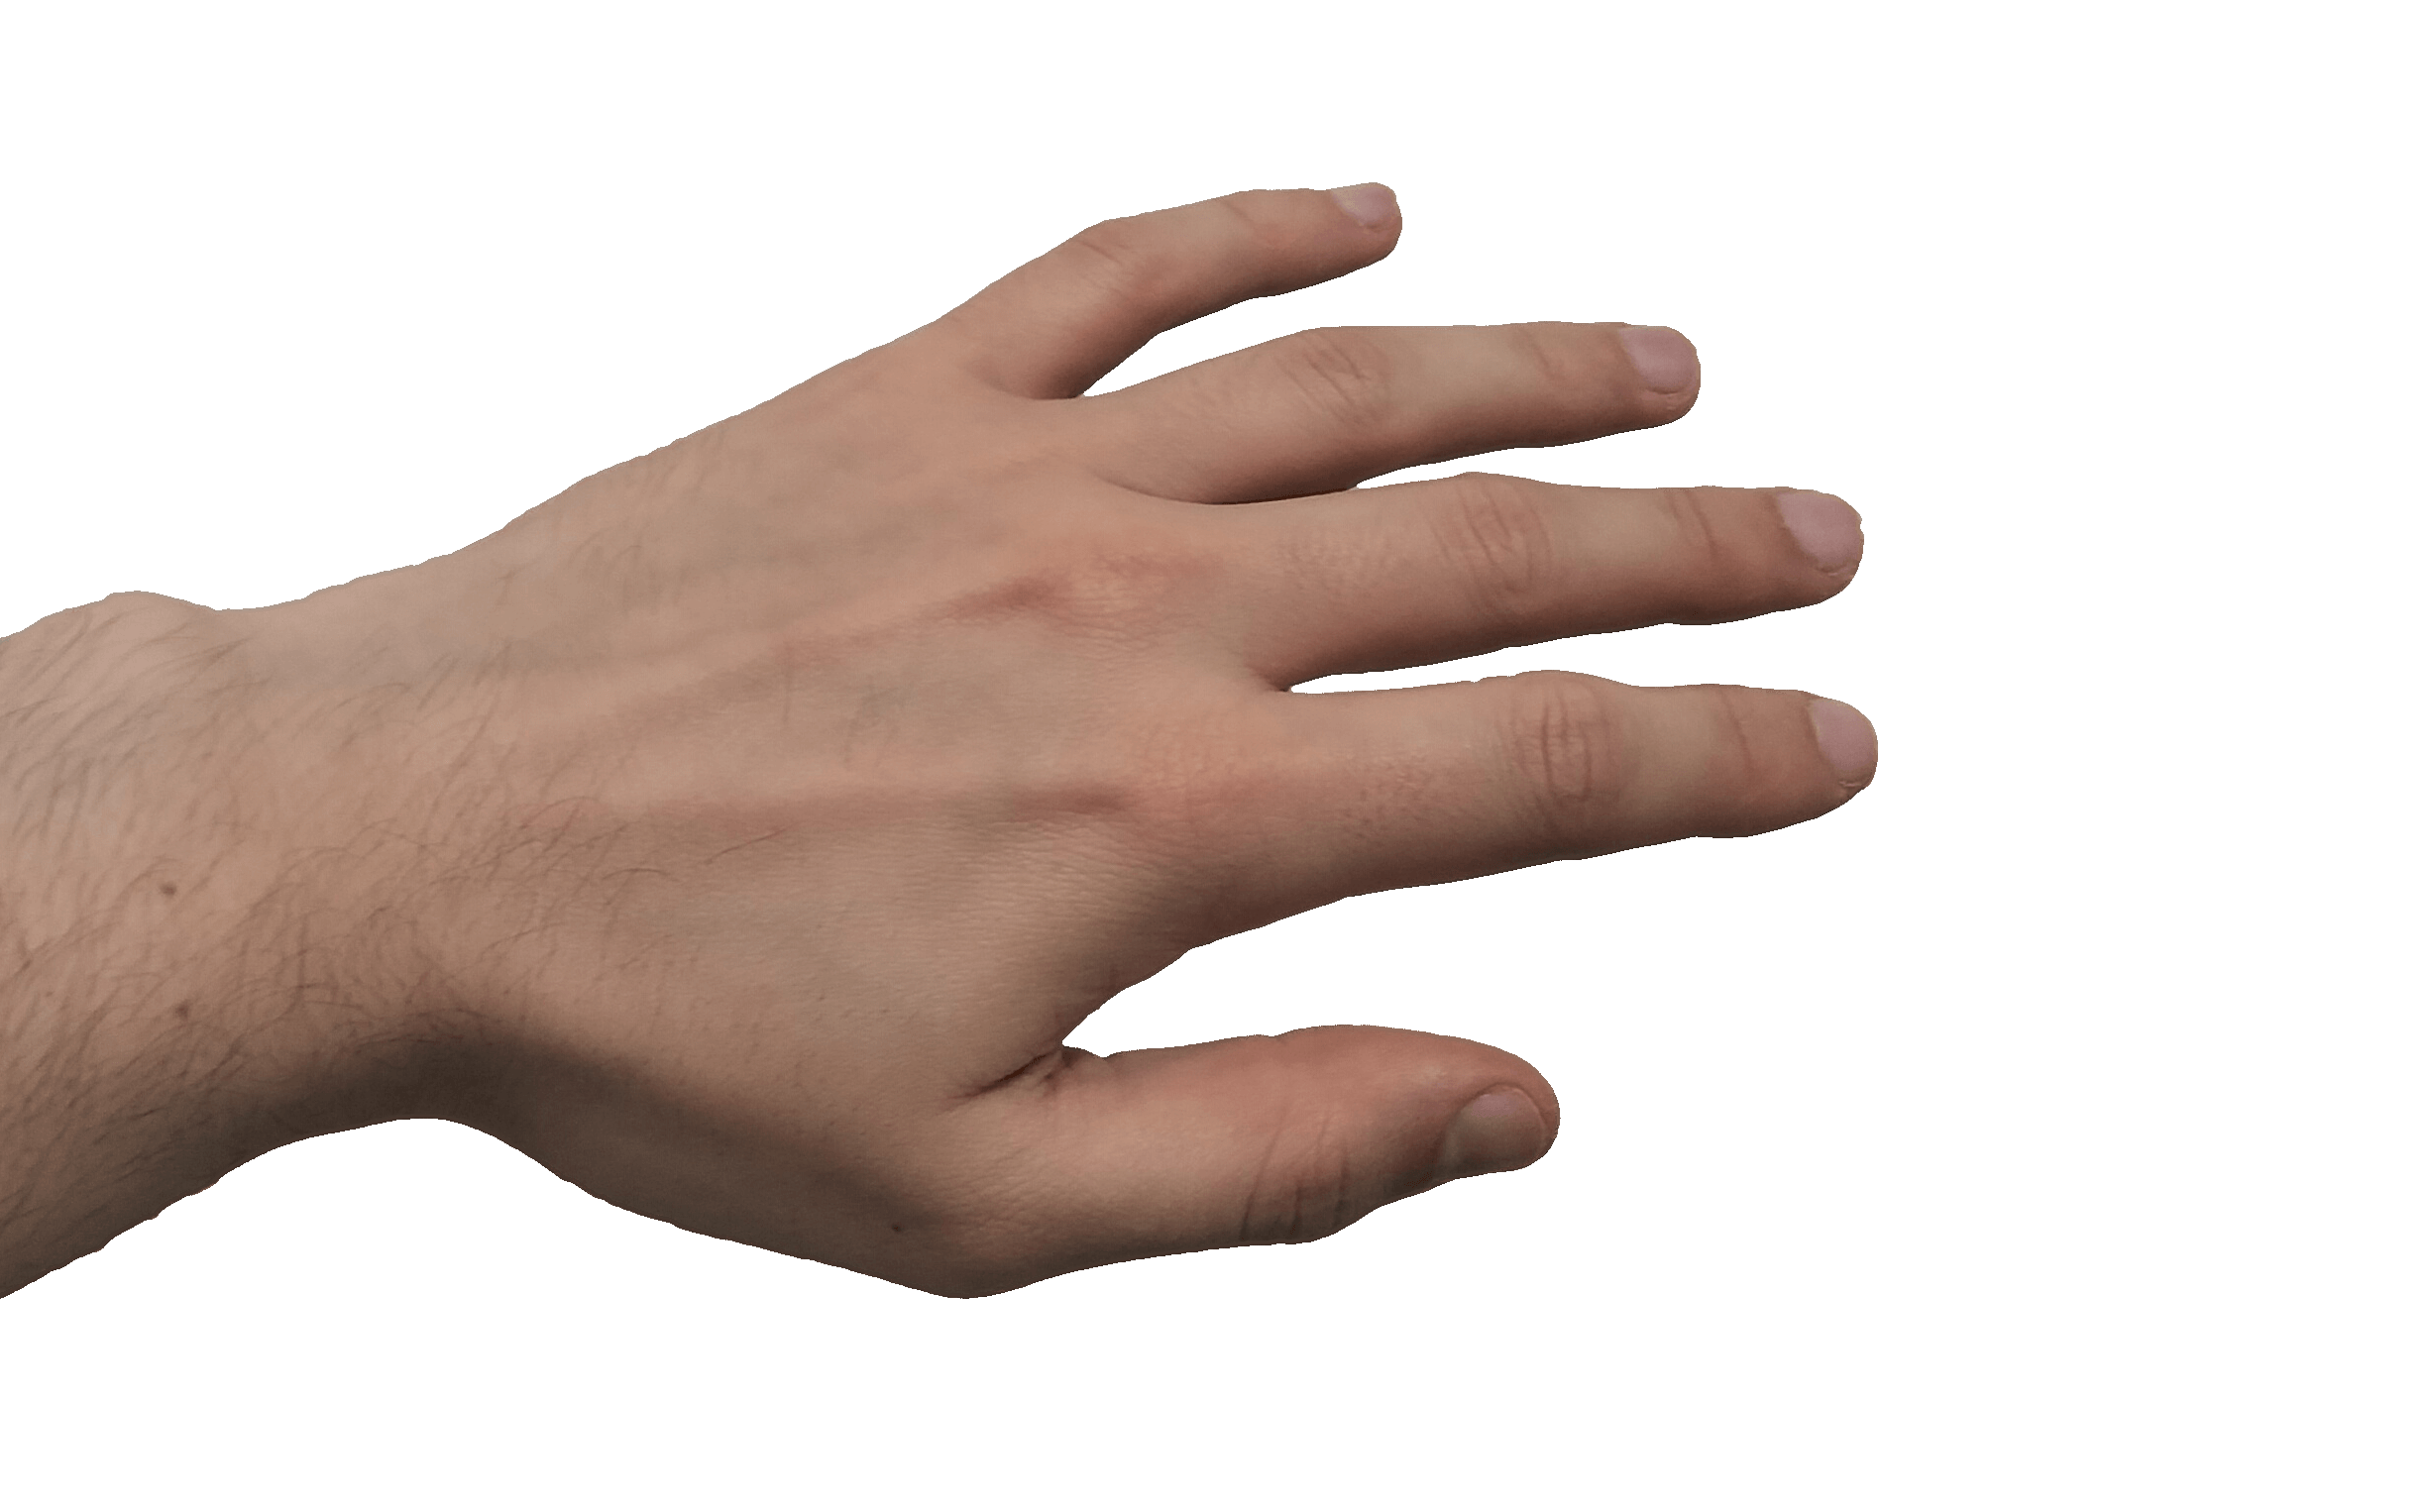
\includegraphics[width=20cm]{hand-compressed.png}};
    \end{pgfonlayer}
    \begin{scope}[x={(image.south east)},y={(image.north west)}]
        \tikzset{
            marker/.style={
                draw=black,
                circle,
                minimum width=0.6cm,
                },
            label/.style={
                anchor=south west,
                inner sep=2pt,
                },
        }
        \node[marker] (wrist_mark) at (0.14,0.47) {};
        \node[label] (wrist_text) at (0.33, 0.005+0.065*0) {Wrist (2 df.) + Forearm rotation (1 df.) };
        \begin{pgfonlayer}{bg}
            \draw[-] (wrist_mark) -- (wrist_text.south west);
        \end{pgfonlayer}
        \draw[-] (wrist_text.south west) -- (wrist_text.south east);


        \node[marker,save path=\thumpmcpmark] (thumb_mcp_mark) at (0.39,0.19) {};
        \node[label] (thumb_mcp_text) at (0.75, 0.005+0.065*1) {Thumb MCP (1 df.)};
        \begin{pgfonlayer}{bg}
            \draw[-] (thumb_mcp_mark) -- (thumb_mcp_text.south west);
        \end{pgfonlayer}
        \draw[-] (thumb_mcp_text.south west) -- (thumb_mcp_text.south east);

        \node[marker] (thumb_cmc_mark) at (0.25,0.25) {};
        \node[label] (thumb_cmc_text) at (0.75, 0.005+0.065*0) {Thumb CMC (2 df.)};
        \begin{pgfonlayer}{bg}
            \draw[dotted] (thumb_cmc_mark) -- (thumb_cmc_text.south west);
            \clip[use path=\thumpmcpmark,reverseclip];
            \draw[-] (thumb_cmc_mark) -- (thumb_cmc_text.south west);
        \end{pgfonlayer}
        \draw[-] (thumb_cmc_text.south west) -- (thumb_cmc_text.south east);

        \node[marker] (thumb_ip_mark) at (0.53,0.22) {};
        \node[label] (thumb_ip_text) at (0.75, 0.005+0.065*2) {Thumb IP (1 df.)};
        \begin{pgfonlayer}{bg}
            \draw[-] (thumb_ip_mark) -- (thumb_ip_text.south west);
        \end{pgfonlayer}
        \draw[-] (thumb_ip_text.south west) -- (thumb_ip_text.south east);

        \node[marker] (index_mcp_mark) at (0.5,0.48) {};
        \node[label] (index_mcp_text) at (0.8, 0.005+0.065*3) {Index MCP (2 df.)};
        \begin{pgfonlayer}{bg}
            \draw[-] (index_mcp_mark) -- (index_mcp_text.south west);
        \end{pgfonlayer}
        \draw[-] (index_mcp_text.south west) -- (index_mcp_text.south east);

        \node[marker,save path=\indexpipmark] (index_pip_mark) at (0.64,0.51) {};
        \node[label] (index_pip_text) at (0.8, 0.005+0.065*4) {Index PIP (1 df.)};
        \begin{pgfonlayer}{bg}
            \draw[-] (index_pip_mark) -- (index_pip_text.south west);
        \end{pgfonlayer}
        \draw[-] (index_pip_text.south west) -- (index_pip_text.south east);

        \clip[use path=\indexpipmark,reverseclip];
        \node[marker,save path=\indexdipmark] (index_dip_mark) at (0.715,0.52) {};
        \node[label] (index_dip_text) at (0.8, 0.005+0.065*5) {Index DIP (1 df.)};
        \begin{pgfonlayer}{bg}
            \draw[-] (index_dip_mark) -- (index_dip_text.south west);
        \end{pgfonlayer}
        \draw[-] (index_dip_text.south west) -- (index_dip_text.south east);

        \node[marker,save path=\midmcpmark] (mid_mcp_mark) at (0.46,0.64) {};
        \node[label] (mid_mcp_text) at (0.825, 0.005+0.065*6) {Middle MCP (2 df.)};
        \begin{pgfonlayer}{bg}
            \draw[dotted] (mid_mcp_mark) -- (mid_mcp_text.south west);
            \clip[use path=\indexpipmark,reverseclip];
            \clip[use path=\indexdipmark,reverseclip];
            \draw[-] (mid_mcp_mark) -- (mid_mcp_text.south west);
        \end{pgfonlayer}
        \draw[-] (mid_mcp_text.south west) -- (mid_mcp_text.south east);

        \node[marker,save path=\middipmark] (mid_dip_mark) at (0.70,0.65) {};
        \node[label] (mid_dip_text) at (0.825, 0.005+0.065*8) {Middle DIP (1 df.)};
        \begin{pgfonlayer}{bg}
            \draw[-] (mid_dip_mark) -- (mid_dip_text.south west);
        \end{pgfonlayer}
        \draw[-] (mid_dip_text.south west) -- (mid_dip_text.south east);

        \clip[use path=\midmcpmark,reverseclip];
        \node[marker,save path=\ringmcpmark] (ring_mcp_mark) at (0.43, 0.70) {};
        \node[label] (ring_mcp_text) at (0.825, 0.005+0.065*9) {Ring MCP (2 df.)};
        \draw[-] (ring_mcp_text.south west) -- (ring_mcp_text.south east);

        \node[marker,save path=\midpipmark] (mid_pip_mark) at (0.62,0.64) {};
        \node[label] (mid_pip_text) at (0.825, 0.005+0.065*7) {Middle PIP (1 df.)};
        \begin{pgfonlayer}{bg}
            \draw[dotted] (mid_pip_mark) -- (mid_pip_text.south west);
            \draw[dotted] (ring_mcp_mark) -- (ring_mcp_text.south west);
            \clip[use path=\middipmark,reverseclip];
            \draw[-] (mid_pip_mark) -- (mid_pip_text.south west);
            \clip[use path=\midpipmark,reverseclip];
            \draw[-] (ring_mcp_mark) -- (ring_mcp_text.south west);
        \end{pgfonlayer}
        \draw[-] (mid_pip_text.south west) -- (mid_pip_text.south east);


        \node[marker, save path=\ringdipmark] (ring_dip_mark) at (0.635, 0.76) {};
        \node[label] (ring_dip_text) at (0.825, 0.005+0.065*11) {Ring DIP (1 df.)};
        \begin{pgfonlayer}{bg}
            \draw[-] (ring_dip_mark) -- (ring_dip_text.south west);
        \end{pgfonlayer}
        \draw[-] (ring_dip_text.south west) -- (ring_dip_text.south east);

        \node[marker,save path=\ringpipmark] (ring_pip_mark) at (0.55, 0.76) {};
        \node[label] (ring_pip_text) at (0.825, 0.005+0.065*10) {Ring PIP (1 df.)};
        \begin{pgfonlayer}{bg}
            \draw[dotted] (ring_pip_mark) -- (ring_pip_text.south west);
            \draw[-] (ring_pip_mark) -- (ring_pip_text.south west);
        \end{pgfonlayer}
        \draw[-] (ring_pip_text.south west) -- (ring_pip_text.south east);

        \node[marker,save path=\pinkypipmark] (pinky_pip_mark) at (0.46, 0.835) {};
        \clip[use path=\pinkypipmark,reverseclip];
        \node[marker,save path=\pinkydipmark] (pinky_dip_mark) at (0.515, 0.86) {};
        \node[label] (pinky_dip_text) at (0.8, 0.005+0.065*14) {Pinky DIP (1 df.)};
        \begin{pgfonlayer}{bg}
            \draw[-] (pinky_dip_mark) -- (pinky_dip_text.south west);
        \end{pgfonlayer}
        \draw[-] (pinky_dip_text.south west) -- (pinky_dip_text.south east);

        \node[label] (pinky_pip_text) at (0.8, 0.005+0.065*13) {Pinky PIP (1 df.)};
        \begin{pgfonlayer}{bg}
            \draw[dotted] (pinky_pip_mark) -- (pinky_pip_text.south west);
            \clip[use path=\pinkydipmark,reverseclip];
            \draw[-] (pinky_pip_mark) -- (pinky_pip_text.south west);
        \end{pgfonlayer}
        \draw[-] (pinky_pip_text.south west) -- (pinky_pip_text.south east);

        \clip[use path=\ringmcpmark,reverseclip];
        \node[marker] (pinky_mcp_mark) at (0.38, 0.75) {};
        \node[label] (pinky_mcp_text) at (0.8, 0.005+0.065*12) {Pinky MCP (2 df.)};
        \begin{pgfonlayer}{bg}
            \draw[dotted] (pinky_mcp_mark) -- (pinky_mcp_text.south west);
            \clip[use path=\ringpipmark,reverseclip];
            \clip[use path=\pinkypipmark,reverseclip];
            \clip[use path=\ringdipmark,reverseclip];
            \draw[-] (pinky_mcp_mark) -- (pinky_mcp_text.south west);
        \end{pgfonlayer}
        \draw[-] (pinky_mcp_text.south west) -- (pinky_mcp_text.south east);
    \end{scope}
\end{tikzpicture}
\end{document}
